\subsection{Serialize RAW Data to Local Disk}

The first step of experiments are serialize various complex objects and the write into a file in disk. In this experiment, the raw tweet data set read line-by-line and convert to a objects. The serialization tasks for each of the thirteen implementation method run. In the serialization process each object serialized or copy the final serialization result into $256KB$ pages and the objects indexed in separate file. 

\subsubsection{Results}

In Figure \ref{fig:exp_serialization_bar}, we show, for each of the thirteen implementations, for both $taskset$ TRUE and FALSE the total running time required as a function of the number of Tweet objects write experiments. In the figure where the
performance differences are easier to see; we also breakdown
the total time into I/O and CPU.
\begin{figure}
	\centering
	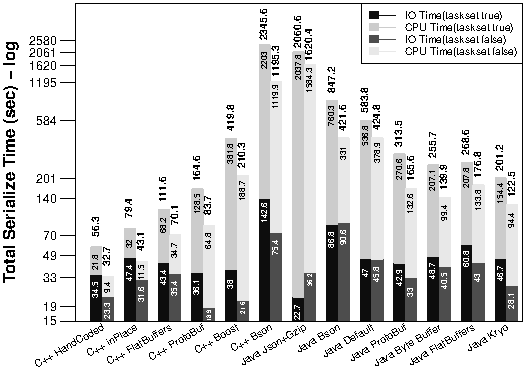
\includegraphics[width=\columnwidth,height=2.5in,keepaspectratio]{../../RScripts/Experiment_SerializeObjects_Bar.pdf}
	\caption{Serialize Objects for 5M Tweets}
	\label{fig:exp_serialization_bar}
\end{figure}

\subsubsection{Discussion}
